\section{Results}
\label{sec:results}

%==========================================================================
% TODO: PÁRRAFO INICIAL - Resumen de la sección
%==========================================================================
% [AQUÍ FALTA: Un párrafo breve (2-3 oraciones) que anticipe la estructura
% de los resultados. Ayuda al revisor a navegar la sección.
%
``We present our findings in four parts. First, we validate the baseline dynamics and classical receptive field properties of the model \commentcd{Cual modelo?}. Second, we compare surround suppression across the three architectural configurations. Third, we demonstrate that only the competitive V2 architecture reproduces the $\sim$75\% suppression observed in vivo, and we confirm via virtual ablation that this effect is driven by hierarchical competition. commentcd{ESTO DE VERDAD DE MOSTRARA AQUI Finally, we show that perturbing the E/I balance replicates schizophrenia-linked biomarkers, establishing the model's translational relevance.''} 

%==========================================================================
% \subsection{Spatial Summation and Classical Receptive Field Characterization}
\label{sec:results_crf}
%==========================================================================
\textbf{4.1 Spatial Summation and Classical Receptive Field Characterization.} We first validated the stability of the model in resting state and then the CRF responses. In the absence of targeted stimuli, the network maintained an asynchronous-irregular firing regime with stable baseline rates (e.g., $\sim 0.5$ Hz in superficial layer L2/3 and $\sim 6.2$ Hz in L5, confirming that the introduction of inter-columnar and inter-areal connectivity did not induce pathological oscillations. To characterize the CRF, we evaluated the network's response to variations in stimulus contrast, simulated by parametrically increasing the firing rate of the topographically aligned thalamic afferents (5, 10, 20, and 30 Hz). The model exhibited a monotonic, contrast-dependent scaling of firing rates, particularly prominent in the primary thalamorecipient L4 and the superficial layer L2/3. Furthermore, to ensure spatial specificity, a 20 Hz optimal stimulus was delivered exclusively to the central microcolumn (vertical preference). While the stimulated central column responded vigorously, the spatially distant peripheral column (horizontal preference) remained at baseline firing levels. This demonstrated that local horizontal connections effectively mediate lateral inhibition, preventing spurious horizontal propagation of strong sensory activation and preserving the spatial acuity of the CRF.

%==========================================================================
% TODO: FIGURA DE VALIDACIÓN DEL CRF
%==========================================================================
% [AQUÍ FALTA: Referencia a una figura que muestre:
%   - PSTH de la columna central vs periférica durante estimulación focal
%   - Curva contraste-respuesta (firing rate vs thalamic input)
%   - Tasas basales espontáneas por capa
%
\commentcd{No supe cual figura es esta.} ``Figure~\ref{fig:crf_validation} summarizes the baseline and CRF characterization. Panel A shows the spontaneous firing rates across layers, Panel B displays the contrast-response function, and Panel C confirms the spatial specificity of the CRF response.''
\begin{figure}[t]
  \centering
  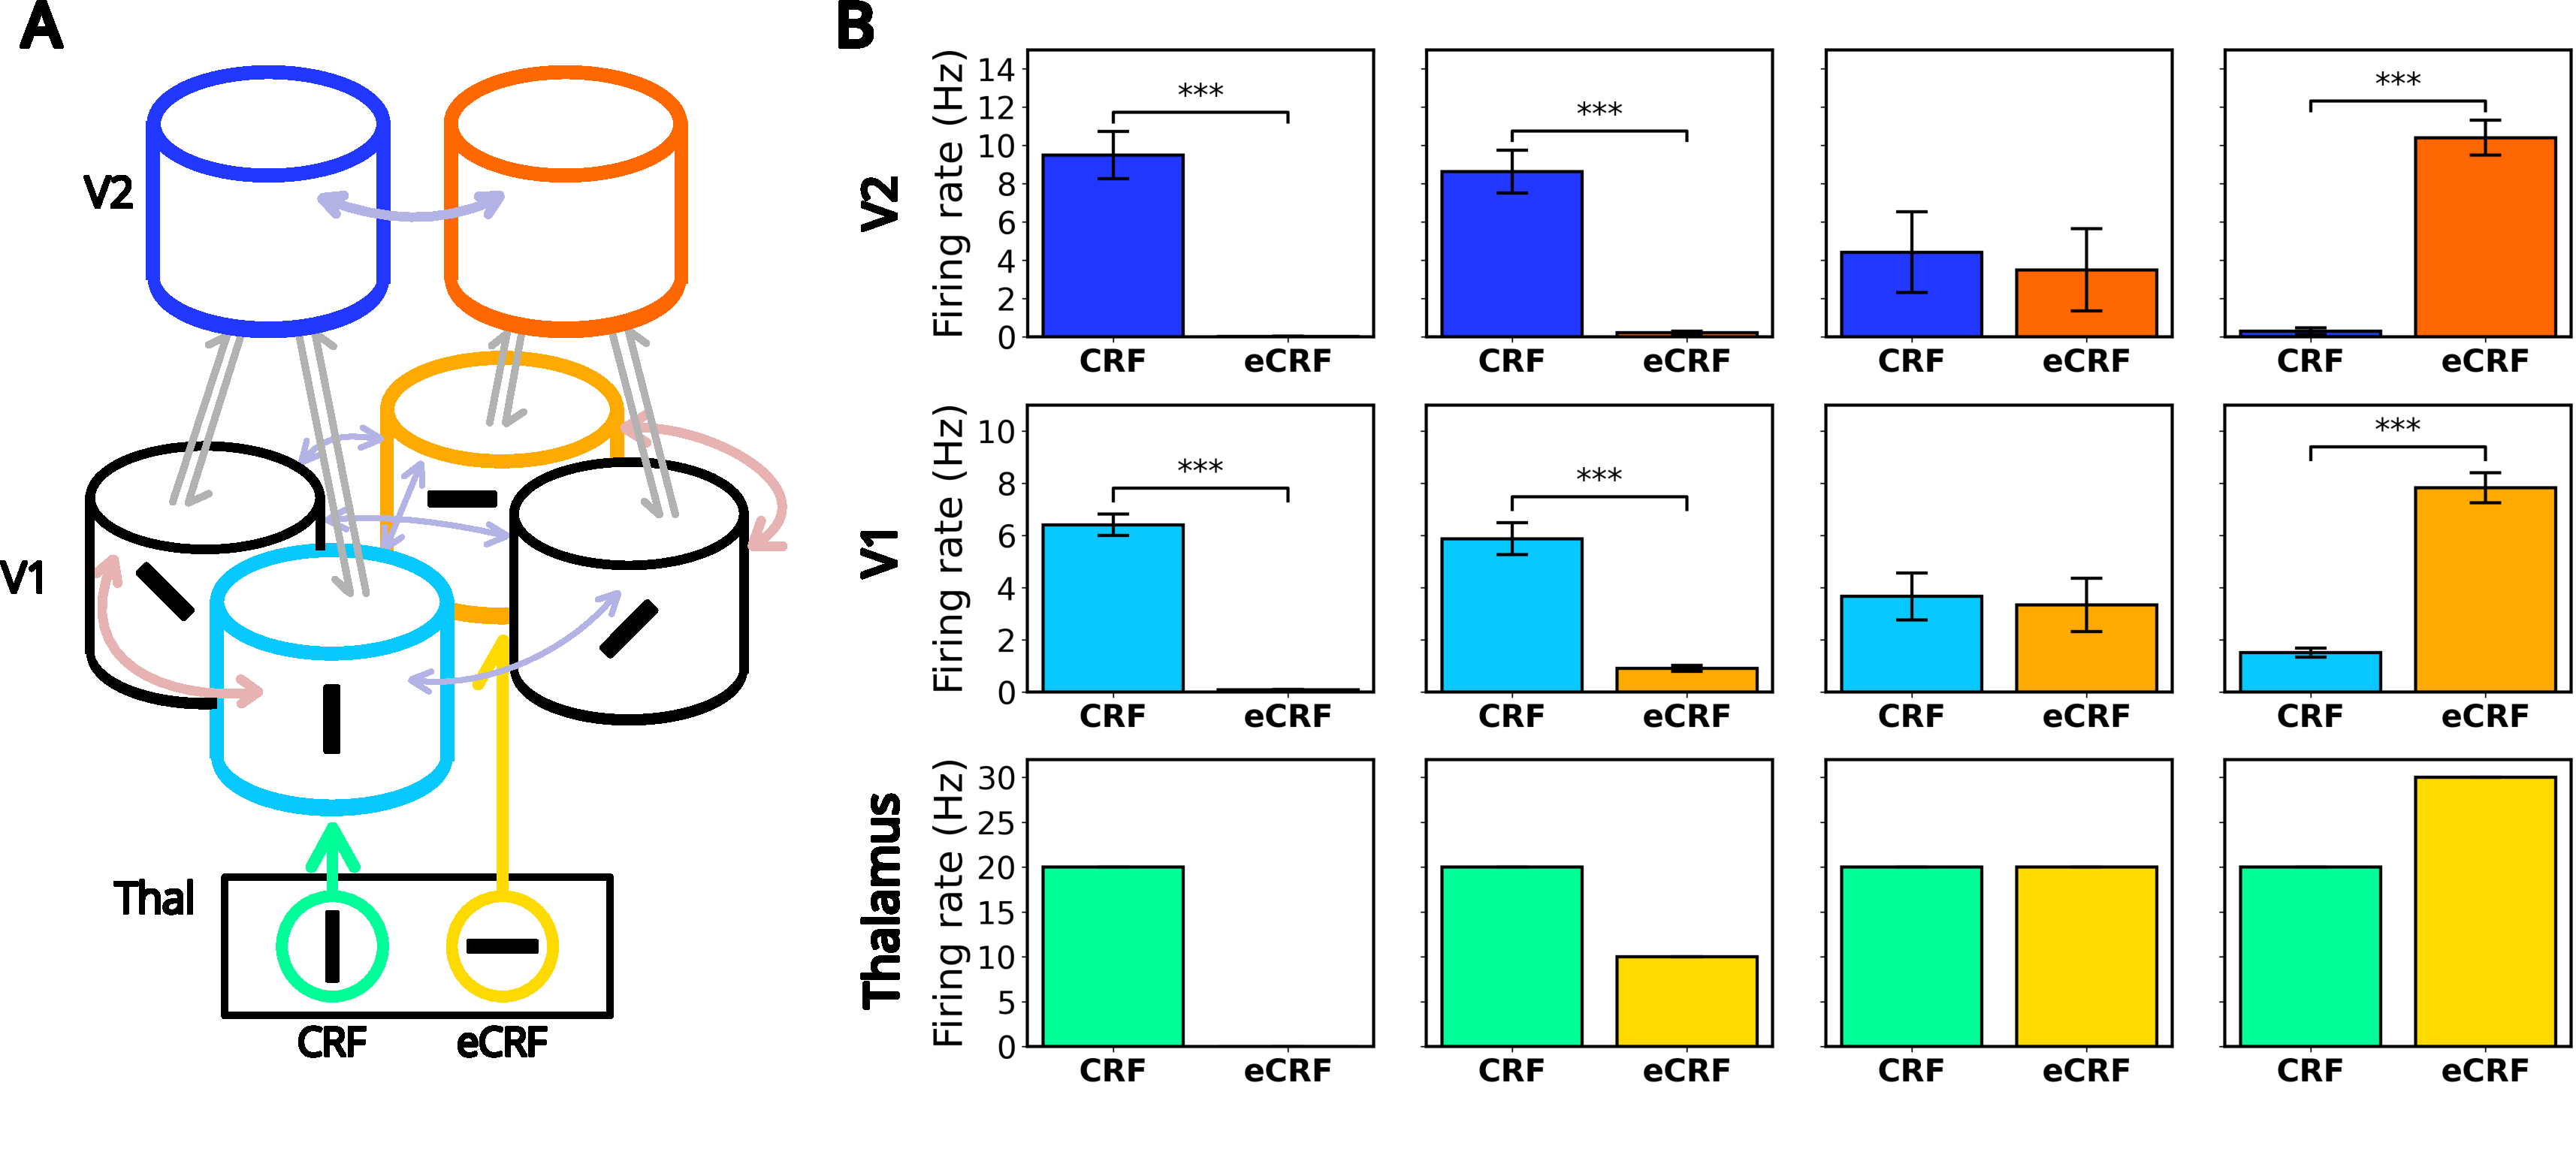
\includegraphics[width=\textwidth]{img/results.pdf}
  \caption{%
    Architectural configurations compared in this study. \commentcd{De nuevo se me confundió la B}
  }
  \label{fig:architectures}
\end{figure}
%==========================================================================
% \subsection{Comparison of Architectural Configurations for Surround Suppression}
\label{sec:results_comparison}
%==========================================================================


\textbf{4.2 Comparison of Architectural Configurations for Surround Suppression.} To systematically evaluate the structural substrates of eCRF effects, we tested the network under a dual-stimulus contextual protocol. A central optimal stimulus, followed by an asynchronous peripheral stimulus of varying intensities. \commentcd{Acá falta alguna estadística.}

We compared the magnitude of surround suppression across three distinct topological configurations. In the first configuration (V1 lateral connections only), the peripheral stimulus induced only a mild suppression. Under the highest contextual contrast (30 Hz), the L2/3 excitatory populations retained $63.3\% \pm 4.4\%$ of their peak CRF activity (equivalent to $\sim$36.7\% suppression). Furthermore, L5 neurons showed virtually no suppressive modulation. This indicated that while intra-areal lateral connectivity contributes to contextual modulation, it is insufficient to replicate the high-magnitude suppression observed \textit{in vivo}.

The second configuration incorporated a single, global V2 module to test the hypothesis of non-specific top-down feedback. While this architecture successfully attenuated L5 activity---consistent with the anatomical targeting of feedback projections to infragranular layers---it failed to suppress L2/3. In fact, L2/3 activity remained at $84.0\% \pm 8.9\%$ of its CRF baseline. Analysis of the V2 module revealed that it acted as a linear integrator, indiscriminately pooling feedforward inputs from both the central and peripheral V1 columns without undergoing internal competition. Consequently, the feedback signal acted more as an excitatory gain amplifier rather than a selective suppressive filter.

%==========================================================================
% TODO: FIGURA COMPARATIVA DE LAS TRES ARQUITECTURAS
%==========================================================================
% [AQUÍ FALTA: Referencia a la figura principal del paper. Debe mostrar:
%   - Panel A: Esquema de cada arquitectura (simplificado)
%   - Panel B: PSTH de L2/3 y L5 para cada arquitectura durante el protocolo
%              center + surround a 30 Hz
%   - Panel C: Bar plot del suppression index para cada arquitectura
%   - Panel D: suppression index en función de la intensidad del surround
%              (10, 20, 30 Hz) para cada arquitectura
%
Results from the third architectural configurations was the only that achieves deep suppression in both superficial and deep layers. Figure~\ref{fig:architectures} presents a comprehensive comparison of the three configurations, the PSTHs reveal that  Configurations~1 and~2 show either weak or layer-incomplete modulation. The suppression index quantifies this difference, Table~\ref{tab:suppression_summary}, reaching $\sim$77\% only in the competitive V2 architecture.

%==========================================================================
% TODO: TABLA RESUMEN DE SUPRESIÓN POR ARQUITECTURA
%==========================================================================
% [AQUÍ FALTA: Una tabla que resuma los valores numéricos clave. Muy útil
% para el revisor que quiere ver los números rápidamente.
%


\begin{table}[t]
  \caption{Suppression index by architecture and layer \commentcd{por què hay solo 2 capas y solo una esta cuantificada? es confuso verlo asi.}}
  \label{tab:suppression_summary}
  \centering
  \begin{tabular}{lccc}
    \toprule
    Architecture & L2/3 Suppression & L5 Suppression & Reaches $\sim$75\%? \\
    \midrule
    Config.~1 (V1 lateral only)   & $\sim$36.7\% & $\sim$0\%    & No \\
    Config.~2 (Linear V2 feedback) & $\sim$16.0\% & Moderate    & No \\
    Config.~3 (Competitive V2)     & $\sim$77.1\% & Strong      & Yes \\
    \bottomrule
  \end{tabular}
\end{table}

%==========================================================================
% \subsection{Robust Suppression via Hierarchical Competitive Dynamics}
\label{sec:results_wta}
%==========================================================================
\textbf{4.3 Robust Suppression via Hierarchical Competitive Dynamics. }The integration of a hierarchically segregated, competitive V2 architecture (Configuration 3) fundamentally altered the network's dynamics. In this design, two distinct V2 modules---each aligned to specific feature columns in V1---interacted via strong, reciprocal inhibitory connections. Under the eCRF stimulation protocol, the activation of the peripheral column triggered a robust winner-take-all dynamic in V2. The peripheral V2 module's activity surged, thereby actively suppressing the central V2 module, whose firing rate plummeted to near baseline levels ($\sim 1$ Hz). This highly selective refinement of the feedback signal profoundly modulated V1. In the central V1 microcolumn, L2/3 activity was suppressed to $22.9\% \pm 8.3\%$ of its maximum CRF response. This equates to a suppression index of approximately $77\%$, which quantitatively replicates the $\sim 75\%$ suppression magnitude historically recorded in macaque V1 (e.g., \citet{Busse2009}).

\commentcd{Estos resultados se podrían poner en el anexo} To conclusively isolate the source of this modulation, we performed virtual ablation experiments. Completely removing the horizontal lateral connections within V1 did not abolish the surround suppression effect. This remarkable resilience demonstrates that the top-down feedforward-feedback (FF-FB) loop, equipped with competitive inter-areal dynamics in higher visual cortices, is both necessary and sufficient to mediate robust far-surround suppression, overcoming the spatial and temporal limitations of slow, intra-areal lateral axons.

%==========================================================================
% TODO: FIGURA DEL WTA EN V2
%==========================================================================
% [AQUÍ FALTA: Una figura mostrando la dinámica del WTA. Debe incluir:
%   - Panel A: PSTH de los dos módulos de V2 (central vs periférico)
%              durante el protocolo, mostrando el cruce (central cae,
%              periférico sube)
%   - Panel B: Raster plot de la población de V2 central y periférica
%   - Panel C: PSTH de L2/3 y L5 en V1 para la Configuración 3, con y sin
%              conexiones laterales en V1 (ablación)
%
`\commentcd{¿cual figura es esta?} `Figure~\ref{fig:wta_dynamics} captures the winner-take-all transition in V2 and its consequence for V1 suppression. Panel A shows the firing rates of the two V2 modules diverging sharply upon peripheral stimulation. Panel B presents a raster plot illustrating the silencing of the central V2 population. Panel C confirms that V1 lateral ablation does not rescue the suppressed response, demonstrating the sufficiency of the hierarchical competitive loop.''

%==========================================================================
% TODO: ANÁLISIS DE SENSIBILIDAD DE LA FUERZA INHIBITORIA EN V2
%==========================================================================
% [AQUÍ FALTA: Un análisis que muestre cómo cambia la supresión al variar
% la fuerza de las conexiones inhibitorias recíprocas en V2. Esto demuestra
% robustez y puede revelar un punto crítico donde emerge el WTA.
%
\commentcd{Aca tb me perdi, donde estan estos resultados.}``To further characterize the dependence of surround suppression on the strength of V2 lateral inhibition, we systematically varied the weight of reciprocal inhibitory connections between V2 modules from 0\% to 150\% of the baseline value. As shown in Figure~\ref{fig:sensitivity}, the suppression index exhibits a sharp nonlinear transition, with robust WTA dynamics emerging only above a critical inhibitory strength of approximately 60\% of baseline. Below this threshold, the V2 modules behave essentially as independent integrators and suppression remains weak. This analysis confirms that strong lateral inhibition in higher cortex is not merely beneficial but \emph{necessary} for the emergence of physiological levels of surround suppression.''
